\chapter{Moving Relays}
\section{Mobility Model}
In this section we describe two mobility models that are commonly used to study the effects of
mobility in cellular networks. One is the classical random waypoint (RWP) model and the other
is the RWP mobility model proposed in \cite{lin}. In classical RWP, the node selects the destination, called waypoint, uniformly from the whole domain and velocity is selcted from a uniform distribution. The node then moves from current waypoint to next waypoint along a straight line at the velocity selected. The distance it travels in doing so is called \textit{transition length} and the time \textit{transition time}. We will not use the classical RWP model as the
transition lengths in this model are of the order of size of domain which is not 
the case in mobility of relays in cellular networks. Also, as noted in \cite{lin}, Rayleigh RWP compares well with synthetic Levy Walk, which is constructed from real mobility trajectories, in terms of CDFs of transition length and direction switch rates than classical RWP model. 
\subsection{Rayleigh RWP Model}
We define mobility more formally and introduce the model proposed in \cite{lin}. The $n$th transition of a node can be denoted by the parameters set $(\mathbf{X}_{n-1},\mathbf{X}_n, V_n, S_n) $. $X_{n-1}$ denotes the starting waypoint and $X_N$ denotes the destination. In addition to the transition time which can be obtained from velocity $V_n$, pause time or thinking time ($S_n$) at destination can also be included in the description of mobility. 
Different mobility models can be distinguished by the distribution of transition length($L_n = \|\mathbf{X}_{n-1} - \mathbf{X}_n \|$) and the distribution of angle made by the vector
$\mathbf{X}_n - \mathbf{X}_{n-1}$ w.r.t x-axis. 
In Rayleigh RWP, the angle is chosen uniformly from $[0,2\pi]$ and the transition length is rayleigh distributed with parameter $\lambda$. 
\begin{equation}
	P(L > l) = exp(-\lambda \pi l^2), l \geq 0
\end{equation}
We set $V_n\equiv v$ and $S_n$ to 0 . What the above selection of distributions means is 
that when the node is at waypoint $\mathbf{X}_{n-1}$, a homogenous Poisson Point Process $\phi$ of intensity $\lambda$ is generated and the nearest point in the set is chosen as the next waypoint $\mathbf{X}_n$. i.e., $\mathbf{X}_n = \arg \min_{x\in\phi} \| x - \mathbf{X}_{n-1}\|$. This can be proved from the null distribution of PPP. This gives better insight in to the role of parameter $\lambda$. Larger $\lambda$ implies that the points are denser in generated PPP
which in turn means the transition length is shorter. Figure \ref{fig:rwp} shows sample traces
of rayleigh RWP for different $\lambda$. Please note that the figures are scaled differently.

\begin{figure}[h]
    \centering \vspace{-0.1in}
    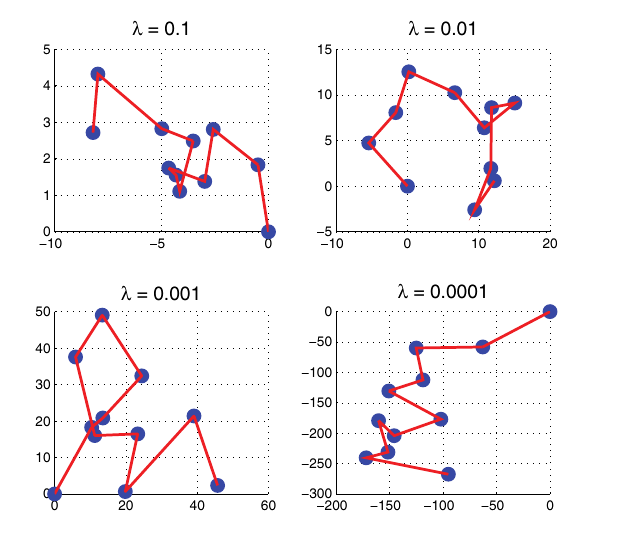
\includegraphics[width=0.6\textwidth]{images/rwpTraces.png}
    \vspace{-20pt} \caption[Sample traces of rayleigh RWP mobility model]{\small The transition	lengths are statistically shorter with larger mobility parameter $\lambda$, and vice
	versa.\footnotemark}
    \label{fig:rwp}
\end{figure}
\footnotetext{Image Source: \cite{lin} Xingqin Lin et al.}
The mean transition length and time are as follows:
\begin{align}
	E[L] &= \frac{1}{2\sqrt{\lambda}} \\[2ex]
	E[T] &= \frac{1}{2v\sqrt{\lambda}}
\end{align}
both of which can be easily derived from distribution of $L$.
\section{Mean Sojourn Time}
Sojourn time is the amount of time a node resides in the region of interest. Calculating the mean sojour time is challenging primarily because it involves finding node distribution during each transition. An expression for  mean sojourn time of a cell user during one movement period starting from origin in a hexagonal cell was given in \cite{lin}. We have to note that
a moving node, on an average, makes atleast two transitions before it leaves
the region. Also, starting from origin implies the node co-exists with BS at
t=0 which is not representative of the distribution of relays/users. Even if we
allow these two assumptions, the problem is still difficult to solve in this
approach as the region has no definite shape like a polygon and finding limits
for integration is tedious. 
	If we know the expected number of transitions $E(N)$ a node mokes before moving out of the
region, then sojourn time can be given by
\begin{equation*}
	S_T = (E(N)-1)E(T) + T_{last}
\end{equation*}
where $T_{last}$ is the time spent inside the region during the last transition. For small $\lambda$, $S_T$ can be approximated to $E(N)E(T)$ and for larger $\lambda$s it can be approximated to $(E(N)-1)E(T)$. Since we already know $E(T)$, what remains to be found is $E(N)$. The 
general form of the expression for $E(N)$ is
\begin{equation*}
	E(N) = \sum_{k=1}^{\infty} k Pr(r,\theta,k)
\end{equation*}
where 
\begin{equation*}
	Pr(r,\theta,k) = \int_{S-A} \int_A \int \ldots \int \int_A f_{X_1/X_0}(x_1/x_0)f_{X_2/X_1}(x_2/x_1)\ldots f_{X_{k+1}/X_{k}}(x_{k+1}/x_{k}) dA_1 dA_2\ldots dA_{k+1}
\end{equation*} is the probability that the node exits the region during $k+1$ th transition. 
$f_{X_n/X_{n-1}}(x_n/x_{n-1})$ is the probability density of the destination $X_n$ given that
the node's current position is $X_{n-1}$. $X_0 = (r,\theta)$ is where the node starts the  movement at t=0. 
As a first step towards finding $E(N)$, let us find the probability with which a node at $(r,\theta)$ leaves the region in one transition.

\section{Leaving in  one transition}
To know whether or not the node is outside the region, we have to find the boundaries it has to cross in each direction. To do this we use plane geometry and trigonometry to find necessary distances and angles.
\subsection{Boundaries of the region}
Consider the figure \ref{fig:rr1}. 
\begin{figure}[h]
    \centering \vspace{-0.1in}
    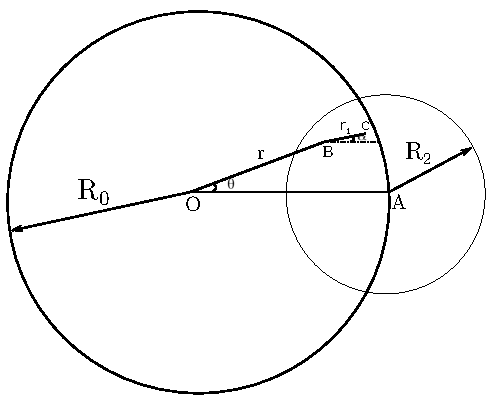
\includegraphics[width=0.6\textwidth]{images/geo1.pdf}
    \vspace{-20pt} \caption[Effect of the proximal Operator]{\small Effect of the Proximal Operator }
    \label{fig:rr1}
\end{figure}
The node starts at $B$ and let $C$ be 
the destination during first transition. $\alpha, r_1$ are chosen according to the mobility 
model described in the previous section. Whether or not $C$ is outside the region depends on
its distance from the circles' centers $O$ and $C$. $OC$ can be found using cosine rule:
$OC^2 = OB^2 + BC^2 - 2 \cdot OB \cdot BC \cdot \cos(\angle CBO)$. $\angle CBO = \pi-\theta+\alpha$ (see figure \ref{fig:ocac}).
\begin{figure}[h]
    \centering \vspace{-0.1in}
    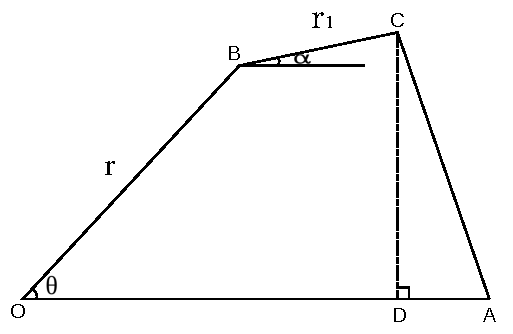
\includegraphics[width=0.6\textwidth]{images/geo2.pdf}
    \vspace{-20pt} \caption[Effect of the proximal Operator]{\small Effect of the Proximal Operator }
    \label{fig:ocac}
\end{figure}

 Therefore, \begin{equation} OC^2 = r^2 + r_1^2 + 2rr_1\cos(\theta-\alpha) \end{equation} To find $AC$, drop a perpendicular from $C$ to the line $OA$ and let the intersection point be $D$ as shown in figure \ref{fig:ocac}. Consider $\bigtriangleup CDA$, 
\begin{align*}
CD &= OB\sin\theta + BC\sin\alpha \\
&= r\sin\theta + r_1\sin\alpha \\
DA &= OA - OB\cos\theta - BC\cos\alpha \\
&= R_0-r\cos\theta-r_1cos\alpha
\end{align*}
Since $\angle CDA = \pi/2$, $AC^2 = CD^2 + DA^2$. $AC$ can therefore be given by 
\begin{equation}
	AC^2 = (r\sin\theta + r_1\sin\alpha)^2 + (R_0-r\cos\theta-r_1cos\alpha)^2
\end{equation}
To find which circle the node crosses first, we also need the angle made by the circle intersections at $B$. Let $\alpha_1$ and $\alpha_2$ be as shown in figures \ref{fig:alpha1} and \ref{fig:alpha2} where $BH$ is a horizontal line. 


\begin{figure}[h]
\centering \vspace{-0.1in}
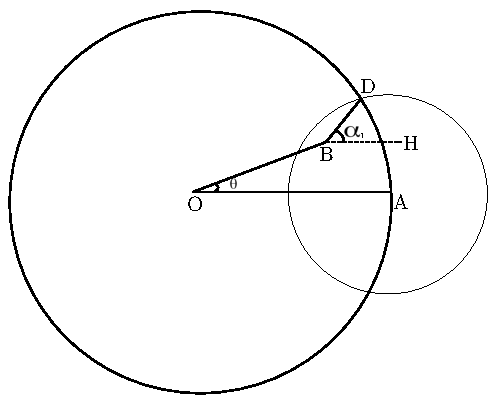
\includegraphics[width=0.6\textwidth]{images/geo3.pdf}
\vspace{-20pt} \caption[Effect of the proximal Operator]{\small Effect of the Proximal Operator }
\label{fig:alpha1}
\end{figure} 
\newpage
In figure \ref{fig:alpha1}, join $OD$ and drop
a perpendicular from $D$ to meet the extension of the $OB$ at $E$. To avoid clutter, let us 
remove the circles and form figure \ref{fig:alpha11}. 
\begin{figure}[h]
\centering \vspace{-0.1in}
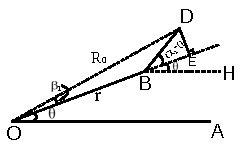
\includegraphics[width=0.6\textwidth]{images/geo4.pdf}
\vspace{-20pt} \caption[Effect of the proximal Operator]{\small Effect of the Proximal Operator }
\label{fig:alpha11}
\end{figure}
Consider $\bigtriangleup DOA$, 
\begin{align*}
	AD^2 &= OD^2 + OA^2 - 2 \cdot OD \cdot OA \cdot \cos(\beta_1+\theta) \\
	R_2^2 &= R_0^2 + R_0^2 - 2R_0^2\cos(\beta_1 + \theta)\\
\end{align*}
\begin{equation}\label{eq:beta1}
	\beta_1 = \cos^{-1}\bigg(1-\frac{R_2^2}{2R_0^2}\bigg) - \theta
\end{equation}
Using $\beta_1$ we can find $\alpha_1$
\begin{align*}
	\tan(\alpha_1 - \theta) &= \frac{DE}{BE} \\[2ex]
							&= \frac{DE}{OE-OB}\\[2ex]
							&= \frac{R_0 \sin\beta_1}{R_0\cos\beta_1 - r} \\[2ex]
	\alpha_1 &= \theta + \tan^{-1}\bigg( \frac{R_0 \sin\beta_1}{R_0\cos\beta_1 - r}\bigg) 
\end{align*}
\begin{figure}[h]
\centering \vspace{-0.1in}
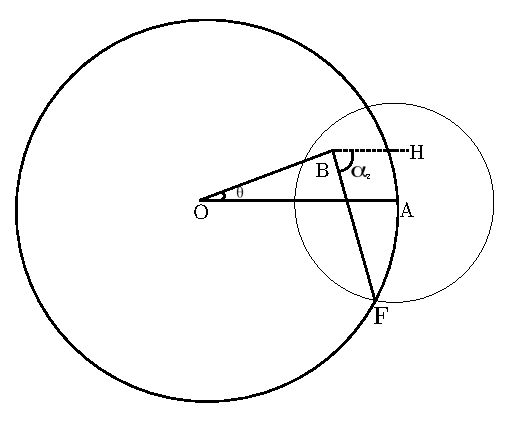
\includegraphics[width=0.6\textwidth]{images/geo5.pdf}
\vspace{-20pt} \caption[Effect of the proximal Operator]{\small Effect of the Proximal Operator }
\label{fig:alpha2}
\end{figure}
$\alpha_2$ and $\beta_2$ are defined in figures \ref{fig:alpha2} and \ref{fig:alpha21}. $\beta_2 = \beta_1 + \theta$ by symmetry. Using expression \ref{eq:beta1} for $\beta_1$, we get

\begin{equation}\label{eq:beta2}
	\beta_2 = \cos^{-1}\bigg(1-\frac{R_2^2}{2R_0^2}\bigg)
\end{equation}

\begin{figure}[h]
\centering \vspace{-0.1in}
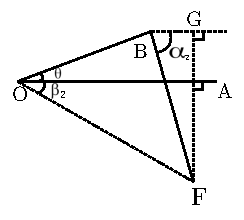
\includegraphics[width=0.6\textwidth]{images/geo6.pdf}
\vspace{-20pt} \caption[Effect of the proximal Operator]{\small Effect of the Proximal Operator }
\label{fig:alpha21}
\end{figure}

To find $\alpha_2$, consider $\bigtriangleup BGF$ in figure \ref{fig:alpha21}

\begin{align*}
	\tan\alpha_2 &= \frac{FG}{GB} \\[2ex]
			  &= \frac{FA+AG}{GB} \\[2ex]
			  &= \frac{R_0 \sin\beta_2 + r\sin\theta}{R_0 \cos\beta_2 - r\cos\theta} \\[2ex]
\Rightarrow \alpha_2 &= \tan^{-1}\bigg( \frac{R_0 \sin\beta_2 + r\sin\theta}{R_0 \cos\beta_2 - r\cos\theta} \bigg) 
\end{align*}

\subsection{Probability}
When $-\alpha_2 < \alpha < \alpha_1$, $C$ is outside the region if $OC^2 > R_0^2$ and for other values of $\alpha$, the node leaves the region if $AC^2 > R_2^2$. The probability of node leaving the region in one transition, let us call it $\rho(r,\theta)$
, is given by
\begin{equation}\label{eq:prob1}
	\rho(r,\theta) = Pr(-\alpha_2 < \alpha < \alpha_1,OC^2 > R_0^2) + Pr(\alpha_1 < \alpha < 2\pi-\alpha_2, AC^2 > R_2^2) \\
\end{equation}
Let us rewrite the above in terms of $r_1$ whose distribution we know.
$AC^2 > R_2^2 \Rightarrow$

\begin{align*}
	(r\sin\theta + r_1\sin\alpha)^2 + (R_0-r\cos\theta-r_1cos\alpha)^2 &> R_2^2 \\
	r_1^2 \sin^2\alpha + r^2\sin^2\theta + 2rr_1\sin\theta\sin\alpha &+ \\ (R_0-r\cos\theta)^2 +
	r_1^2\cos^2\alpha - 2(R_0-r\cos\theta)r_1\cos\alpha - R_2^2 &> 0\\ 
	r_1^2 + 2 r_1 (r\sin\alpha\sin\theta-(R_0-r\cos\theta)\cos\alpha) + r^2\sin^2\theta +
	(R_0-r\cos\theta)^2 -R_2^2 &>0 \\
	r_1^2 + 2(r\cos(\theta-\alpha) - R_0\cos\alpha) r_1 + r^2\sin^2\theta +	(R_0-r\cos\theta)^2 - R_2^2 &> 0 
\end{align*}
The above inequality gives two feasible intervals for $r_1$ one of which is spurious since $r_1 > 0$ and the other is 
\begin{align}\label{ineq:ACcon}
	r_1 > (R_0\cos\alpha - r\cos(\theta-\alpha)) + \sqrt{\big(R_0\cos\alpha-r\cos(\theta-\alpha)\big)^2 + R_2^2 - r^2\sin^2\theta - 	(R_0-r\cos\theta)^2 }
\end{align}
Similar calculations as above will reduce $OC^2 > R_0^2$ to
\begin{align} \label{ineq:OCcon}
	r_1 > -r\cos(\theta-\alpha) + \sqrt{R_0^2 - r^2\sin^2(\theta-\alpha)}
\end{align}
Let us denote the R.H.S of the above two inequalities by $r_{12}$ and $r_{11}$ respectively.
Substituting \ref{ineq:ACcon} and \ref{ineq:OCcon} in \ref{eq:prob1}, we get
\begin{align*}
	\rho(r,\theta) &= Pr(-\alpha_2 < \alpha < \alpha_1,r_1 > r_{11}) + Pr(\alpha_1 < \alpha < 2\pi-\alpha_2, r_1 > r_{12}) \\
	&= \int_{-\alpha_2}^{\alpha_1} \int_{r_{\!_{11}}}^{\infty} f_{r_1,\alpha}(r_1,\alpha)dr_1 d\alpha +  \int^{2\pi-\alpha_2}_{\alpha_1} \int_{r_{\!_{12}}}^{\infty} f_{r_1,\alpha}(r_1,\alpha)dr_1 d\alpha 
\end{align*}
	This is a general expresion that can be used for any mobility model. In case of RWP,
	$r_1$ and $\alpha$ are chosen independently. Therefore, 
	$f_{r_1,\alpha}(r_1,\alpha) = f_{r_1}(r_1)f_{\alpha}(\alpha)$ 
\begin{align*}
	\rho(r,\theta)&= \int_{-\alpha_2}^{\alpha_1} f_{\alpha}(\alpha) \int_{r_{\!_{11}}}^{\infty} f_{r_1}(r_1)dr_1 d\alpha +  \int^{2\pi-\alpha_2}_{\alpha_1} f_{\alpha}(\alpha) \int_{r_{\!_{12}}}^{\infty} f_{r_1}(r_1)dr_1 d\alpha  \\
	&= \int_{-\alpha_2}^{\alpha_1} \frac{1}{2\pi} e^{-\lambda \pi r_{\!_{11}}^2} d\alpha +  \int^{2\pi-\alpha_2}_{\alpha_1} \frac{1}{2\pi} e^{-\lambda \pi r_{\!_{12}}^2} d\alpha
\end{align*}
\newpage
Putting it all together at one place for ease of reference, this is what have about the node's
first transition. \\
The probability with which a 
node at $(r,\theta)$ moves out of the region of interest during the next transition is 
\begin{equation} \label{eq:oneOutProb}
	\rho(r,\theta) = \int_{-\alpha_2}^{\alpha_1} \frac{1}{2\pi} e^{-\lambda \pi r_{\!_{11}}^2} d\alpha +  \int^{2\pi-\alpha_2}_{\alpha_1} \frac{1}{2\pi} e^{-\lambda \pi r_{\!_{12}}^2} d\alpha
\end{equation}
\\
Where
\begin{align*}
	r_{\!_{11}} &= -r\cos(\theta -\alpha) + \sqrt{R_0^2 - r^2\sin^2(\theta - \alpha)} \\
	&\\
	r_{\!_{12}} &= R_0 \cos \alpha - r\cos(\theta - \alpha)  +  \sqrt{[R_0 \cos \alpha - r\cos(\theta-\alpha) ]^2 - r^2\sin^2 \theta - [R_0 - r\cos \theta]^2 + R_2^2} \\
\end{align*}
\begin{align*}
	\beta_1 &= \cos^{-1}\bigg(1-\frac{R_2^2}{2R_0^2}\bigg) - \theta \\
	& \\
		\beta_2 &= \cos^{-1}\bigg(1-\frac{R_2^2}{2R_0^2}\bigg) \\
	& \\
	\alpha_1 &= \theta + \tan^{-1}\bigg( \frac{R_0\sin\beta_1}{R_0\cos\beta_1-r}\bigg)\\
			& \\
			\alpha_2 &= \tan^{-1}\bigg( \frac{r\sin\theta + R_0\sin\beta_2}{R_0cos\beta_2 - r\cos\theta} \bigg)
\end{align*}
